\documentclass[oneside,a4paper,11pt]{book}
\usepackage[utf8]{inputenc}
\usepackage{svg}
\usepackage[italian]{babel}
\usepackage{float}
\usepackage{fancyvrb}
\usepackage{titling}
\usepackage[margin=1in,footskip=0.25in]{geometry}
\usepackage{listings}
\usepackage[DIV=12,BCOR=2mm,headinclude=true,footinclude=false]{typearea}
\usepackage{color, colortbl,xcolor}
\usepackage[hidelinks]{hyperref}
\usepackage{tcolorbox}
\usepackage{chngcntr}
\usepackage{diagbox}
\usepackage{calc}
\usepackage{amssymb}
\usepackage{subcaption}
\usepackage{amsthm}
\usepackage{amsfonts}
\usepackage{mathtools}
\usepackage{parskip}
\usepackage{cancel}
\usepackage{forest}
\usepackage{listings}
\usepackage{mathrsfs}
\usepackage{enumitem}
\usepackage{makecell}
\usepackage{tikz}
\usepackage{pgfplots}
\pgfplotsset{compat=1.18}
\usepackage{pgf-umlsd}
\usepackage{pgf-umlcd}
\usetikzlibrary{shapes.geometric, positioning, circuits.logic.US}
\usepackage{fancyhdr}
\fancypagestyle{plain}{\fancyhf{}\renewcommand{\headrulewidth}{0pt}}
\pagestyle{fancy}
\fancyhf{}% Clear header/footer
\fancyhead[L]{\nouppercase\leftmark}
\fancyhead[R]{\thepage}
\usetikzlibrary{positioning,shapes.geometric,arrows.meta,matrix,automata,decorations.pathmorphing,patterns,decorations.pathreplacing,shapes.multipart,calc,snakes}
\usetikzlibrary{arrows.meta, backgrounds, chains, positioning, shapes.geometric, shapes.multipart, shadows}
\usetikzlibrary{shapes, arrows, positioning}
\tcbuselibrary{skins}
\counterwithin{figure}{section}
%Nuovi comandi
\newcommand\myeq{\stackrel{\mathclap{\normalfont\mbox{def}}}{=}}
\newcommand\prodG{\stackrel{\mathclap{\normalfont\mbox{\tiny{G}}}}{\Longrightarrow}}
%asmthm
\newlength{\marginlabelsep}\setlength{\marginlabelsep}{0.5em}
\newtheoremstyle{italicstyle} %% Name
  {} %% <- Space above (empty = default = \topsep = 8.0pt plus 2.0pt minus 4.0pt)
  {} %% <- Space below (empty = default = \topsep = 8.0pt plus 2.0pt minus 4.0pt)
  {\itshape} %% <- Body font
  {} %% <- Indent amount (empty = no indent, \parindent = just that)
  {\bfseries} %% <- Thm head font
  {} %% <- Punctuation after thm head
  {1pt} %% <- Space after thm head (or " " or \newline) (default: 5pt plus 1pt minus 1pt)
  {\vtop to 0pt{\llap{\thmname{#1}\hskip\marginlabelsep}
                \llap{\thmnumber{#2}\hskip\marginlabelsep}}\thmnote{#3\\}%
  }
\newtheoremstyle{normStyle} %% Name
  {} %% <- Space above (empty = default = \topsep = 8.0pt plus 2.0pt minus 4.0pt)
  {} %% <- Space below (empty = default = \topsep = 8.0pt plus 2.0pt minus 4.0pt)
  {\normalfont} %% <- Body font
  {} %% <- Indent amount (empty = no indent, \parindent = just that)
  {\bfseries} %% <- Thm head font
  {} %% <- Punctuation after thm head
  {1pt} %% <- Space after thm head (or " " or \newline) (default: 5pt plus 1pt minus 1pt)
  {\vtop to 0pt{\llap{\thmname{#1}\hskip\marginlabelsep}
                \llap{\thmnumber{#2}\hskip\marginlabelsep}}\thmnote{#3\\}%
  }
\theoremstyle{italicstyle}
\newtheorem{corollary}{Corollario}[section]
\newtheorem{notazione}{Notazione}[section]
\newtheorem{lemma}{Lemma}[section]
\newtheorem{definizione}{Definizione}[section]
\newtheorem{nota}{Nota}[section]
\newtheorem{exercise}{Esercizio}[section]
\theoremstyle{normStyle}
\newtheorem{exmp}{Esempio}[section]
\newtheorem{theorem}{Teorema}[section]
\newtheorem{proposizione}{Proposizione}[section]
\tcbuselibrary{listings,skins}
\newtcblisting{mylisting}[2][]{
    arc=0pt, outer arc=0pt,
    listing only, 
    title=#2,
    #1,
    listing options= {escapechar=|}
}

\usepackage{color}

\definecolor{pblue}{rgb}{0.13,0.13,1}
\definecolor{pgreen}{rgb}{0,0.5,0}
\definecolor{pred}{rgb}{0.9,0,0}
\definecolor{pgrey}{rgb}{0.46,0.45,0.48}

\usepackage{listings}
\lstset{language=Java,
  showspaces=false,
  showtabs=false,
  breaklines=true,
  showstringspaces=false,
  breakatwhitespace=true,
  commentstyle=\color{pgreen},
  keywordstyle=\color{pblue},
  stringstyle=\color{pred},
  basicstyle=\ttfamily,
  moredelim=[il][\textcolor{pgrey}]{$$},
  moredelim=[is][\textcolor{pgrey}]{\%\%}{\%\%}
}
\newcommand{\myboxedtext}[2][rectangle,draw]{%
    \tikz[baseline=-0.6ex] \node [#1]{#2};}%
%%======================================================================
\title{Ingegneria dei Requisiti}
\author{\textit{Alessio Gjergji}}
\date{}
\begin{document}
\begin{titlingpage}
  \centering
  \vspace*{\stretch{1}}
  \huge
  \textbf{\thetitle}\\[0.5cm]
  \normalsize
  Corso tenuto dal Professor Mariano Ceccato\\[0.5cm]
  Università degli Studi di Verona\\[1cm]
  \large
  \theauthor\\[0.5cm]
  \vspace{\stretch{2}}
\end{titlingpage}
\tableofcontents
\chapter{Introduzione}
\section{Linguaggi di programmazione}
Un linguaggio di programmazione è un linguaggio formale che specifica un
insieme di istruzioni che possono essere usate per produrre un insieme di
output.
Esso è definito da:
\begin{itemize}
    \item \textbf{Sintassi}: specifica la forma delle istruzioni. Ci permette di
    capire quali stringhe sono ammissibili e quali no mediante diversi strumenti come 
    grammatiche, analizzatori lessicali e sintattici, teoria degli automi.
    \item \textbf{Pragmatica}: specifica l'effetto delle istruzioni. Ci permette
    di capire le ragioni per introdurre un nuovo linguaggio e di programmazione 
    invece di utilizzarne uno già esistente.
    \item \textbf{Semantica}: specifica il significato dei programmi scritti nel linguaggio, ovvero il loro 
    comportamento a tempo di esecuzione. Ci permette di capire se due programmi 
    apparentemente diversi sono equivalenti.
\end{itemize}
\subsection{Benefici di una semantica formale}
I benefici dei linguaggi di programmazione diversi, tra cui:
\begin{itemize}
    \item \textbf{Implementazione}: Consente di fornire la specifica (\textit{del comportamento}) 
    dei programmi indipendentemente dalla macchina o dal compilatore utilizzato.
    \item \textbf{Verifica}: una semantica formale consente di ragionare 
    sui programmi e sulle loro proprietà di correttezza.
    \item \textbf{Progettazione di Linguaggio}: spesso una semantica formale consente di 
    scoprire ambiguità all'interno di linguaggi già esistenti. Questo aiuta a progettare 
    nuovi linguaggi in maniera più accurata.
\end{itemize}
\section{Un linguaggio per le espressioni aritmetiche: sintassi}
Definiamo il seguente linguaggio:
\[
    \mathcal{E}\quad ::= \quad n \quad | \quad \mathcal{E} + \mathcal{E} \quad | 
    \quad \mathcal{E} * \mathcal{E} \quad | \quad \dots
\]
dove:
\begin{itemize}
    \item $n$ è lo spazio del dominio dei numerali.
    \item $\mathcal{E}$ è il range del dominio delle espressioni aritmetiche.
    \item $+, x, \dots$ sono simboli del linguaggio.
\end{itemize}
I numerali sono parte della sintassi del nostro linguaggio e non vanno confusi con i numeri
che sono oggetti matematici.
Ciò potrebbe significare che nel nostro linguaggio al posto di $0, 1, \dots$ avremmo 
potuto usare $zero, uno, \dots$ e sarebbero potuti essere uguali.

Nel nostro caso assumiamo che esista una corrispondenza ovvia tra il simbolo ``numerale" (n)
e il numero naturale n. Questo è fatto solo per semplificare la spiegazione. In un
altro contesto, il simbolo ``numeral" 3 potrebbe essere associato al numero 42!

\section{Semantica Operazionale}

La semantica operazionale ha l'obiettivo di valutare un'espressione aritmetica
del linguaggio per ottenere il suo valore numerico associato. Questo può essere
fatto in due modi differenti:

\begin{itemize}
  \item \textbf{Semantica Small-Step (\textit{o strutturale})}: Fornisce un metodo per
  valutare un'espressione passo dopo passo, considerando le azioni intermedie.
  Questo approccio fornisce una valutazione dettagliata dell'espressione.

  \item \textbf{Semantica Big-Step (\textit{o naturale})}: Ignora i passaggi intermedi
  e fornisce direttamente il risultato finale della valutazione dell'espressione. Questo
  approccio semplifica la valutazione, concentrando l'attenzione sul risultato finale.

\end{itemize}
\subsection{Big-Step Semantics}

\begin{tcolorbox}[title = {Valutazione}]  
    $E \Downarrow n$
\end{tcolorbox}
\textbf{Significato}: La valutazione dell'espressione $\mathcal{E}$ produce il numerale $n$.

\begin{tcolorbox}[title = {Assiomi e regole di inferenza}]  
\begin{figure}[H]
    \begin{subfigure}{0.3\textwidth}
    \begin{prooftree}
        \AxiomC{$-$}
        \LeftLabel{(B-Num)}
        \UnaryInfC{$n \Downarrow n$}
    \end{prooftree}
    \end{subfigure}%
    \begin{subfigure}{0.7\textwidth}
    \begin{prooftree}
        \AxiomC{$\mathcal{E}_1 \Downarrow n_1$}
        \AxiomC{$\mathcal{E}_2 \Downarrow n_2$}
        \LeftLabel{(B-Add)}
        \RightLabel{$n_3 = add(n_1, n_2)$}
        \BinaryInfC{$\mathcal{E}_1 + \mathcal{E}_2 \Downarrow n_3$}
    \end{prooftree}
    \end{subfigure}
\end{figure}
\end{tcolorbox}
\textbf{Significato}: 
\begin{itemize}
\item (B-Num): Questo è un assioma che afferma che quando valutiamo un singolo
numero $n$, otteniamo lo stesso numero $n$ come risultato. Questo è il caso
base della valutazione.

\item (B-Add): Questa regola di inferenza afferma che date due espressioni
$\mathcal{E}_1$ e $\mathcal{E}_2$:
\begin{itemize}
  \item Se è il caso che $\mathcal{E}_1 \Downarrow n_1$ (cioè $\mathcal{E}_1$ si valuta a $n_1$) e
  \item È anche il caso che $\mathcal{E}_2 \Downarrow n_2$ (cioè $\mathcal{E}_2$ si valuta a $n_2$),
  allora segue che $\mathcal{E}_1 + \mathcal{E}_2 \Downarrow n_3$, dove $n_3$ è il numerale associato
  al numero $n_3$ tale che $n_3 = add(n_1, n_2)$.
  Si noti che in questa regola, $E1$, $E2$, $n1$, $n2$, $n3$ sono meta-variabili.
\end{itemize}
\end{itemize}
Questa regola (B-Add) ci dice come valutare un'addizione tra due espressioni
$\mathcal{E}_1$ e $\mathcal{E}_2$ nel contesto della semantica big-step. La
regola stabilisce che se possiamo valutare entrambe le espressioni operandi
($\mathcal{E}_1$ e $\mathcal{E}_2$) e otteniamo i numeri $n_1$ e $n_2$ rispettivamente,
allora possiamo calcolare la somma di $\mathcal{E}_1$ e $\mathcal{E}_2$ come $n_3$,
dove $n_3$ è il risultato della somma dei numeri $n_1$ e $n_2$.
Si noti che la funzione di addizione $add$ opera sui numeri, non sui numerali.
\subsection{Small-Step Semantics}

\begin{tcolorbox}[title = {Valutazione}]  
$\mathcal{E}_1 \rightarrow \mathcal{E}_2$

\end{tcolorbox}
\textbf{Significato:} 
Dopo aver eseguito un passo di valutazione su $\mathcal{E}_1$, l'espressione $\mathcal{E}_2$ rimane da valutare.
\begin{tcolorbox}[title = {Assiomi e regole di inferenza}]  
\begin{prooftree}
    \AxiomC{$\mathcal{E}_1 \rightarrow \mathcal{E}_1'$}
    \LeftLabel{(S-Left)}
    \UnaryInfC{$\mathcal{E}_1 + \mathcal{E}_2 \rightarrow \mathcal{E}_1' + \mathcal{E}_2$}
    \end{prooftree}
    
    \begin{prooftree}
    \AxiomC{$\mathcal{E}_2 \rightarrow \mathcal{E}_2'$}
    \LeftLabel{(S-N.Right)}
    \UnaryInfC{$n_1 + \mathcal{E}_2 \rightarrow n_1 + \mathcal{E}_2'$}
    \end{prooftree}
    
    \begin{prooftree}
    \AxiomC{-}
    \LeftLabel{(S-Add)}
    \RightLabel{$n_3 = add(n_1, n_2)$}
    \UnaryInfC{$n_1 + n_2 \rightarrow n_3$}
    \RightLabel{(S-Add)}
\end{prooftree}
\end{tcolorbox}
Fissiamo l'ordine di valutazione da sinistra a destra. Qualcosa di 
simile non è possibile nella big-step semantics, dove le espressioni sono 
valutate in un solo passo.
\subsubsection{La scelta dell'ordine di valutazione}
\begin{tcolorbox}[title = {Assiomi e regole di inferenza}]  
    \begin{prooftree}
        \AxiomC{$\mathcal{E}_1 \rightarrow_{ch} \mathcal{E}_1'$}
        \LeftLabel{(S-Left)}
        \UnaryInfC{$\mathcal{E}_1 + \mathcal{E}_2 \rightarrow_{ch} \mathcal{E}_1' + \mathcal{E}_2$}
        \end{prooftree}
        
        \begin{prooftree}
        \AxiomC{$\mathcal{E}_2 \rightarrow_{ch} \mathcal{E}_2'$}
        \LeftLabel{(S-Right)}
        \UnaryInfC{$\mathcal{E}_1 + \mathcal{E}_2 \rightarrow_{ch} \mathcal{E}_1 + \mathcal{E}_2'$}
        \end{prooftree}
        
        \begin{prooftree}
        \AxiomC{-}
        \LeftLabel{(S-Add)}
        \RightLabel{$n_3 = add(n_1, n_2)$}
        \UnaryInfC{$n_1 + n_2 \rightarrow_{ch} n_3$}
        \RightLabel{(S-Add)}
    \end{prooftree}
\end{tcolorbox}
In questo caso non abbiamo precedenza stabilita per la valutazione delle espressioni.
Regole simili possono essere applicate anche con gli altri operatori.
\subsubsection{Esecuzione della small-step semantics}
La relazione $\rightarrow^k$, per $k \in \mathbb{N}$ è definita per un numero di passi 
di valutazione definito da $k$.
Mentre la relazione $\rightarrow^*$ è definita per un numero non definito di passi di valutazione.
\chapter{Elicitazione dei requisiti}
L'obiettivo comprendere il dominio in cui stiamo lavorando e 
raccogliere e capire i requisiti del software che dovrà essere
implementato. 
\section{Acquisizione della conoscenza}

L'acquisizione della conoscenza è una fase cruciale nel processo di
ingegneria dei requisiti e include diverse attività importanti.

In primo luogo, è essenziale studiare il sistema attuale, noto come sistema
\textit{as-is}. Questo studio comprende la comprensione dell'organizzazione
aziendale (\textit{struttura, dipendenze, obiettivi strategici, politiche, flussi di
lavoro e procedure operative}) e del dominio applicativo (\textit{concetti, obiettivi,
compiti, vincoli e regolamenti}). Inoltre, è necessario analizzare i problemi
esistenti nel sistema attuale, identificandone sintomi, cause e conseguenze.

Un'altra attività chiave è l'analisi delle opportunità tecnologiche e delle
nuove condizioni di mercato, per valutare le possibilità offerte dalle nuove
tecnologie e comprendere come i cambiamenti nelle condizioni di mercato possano
influenzare il sistema.

Identificare gli stakeholder del sistema è fondamentale. Gli stakeholder sono
tutte le parti interessate che hanno un'influenza o sono influenzate dal sistema.
Comprendere le loro esigenze e aspettative è vitale per il successo del progetto.

L'identificazione degli obiettivi di miglioramento per il sistema futuro, noto
come sistema \textit{to-be}, è un'altra attività importante. Questo include
l'analisi dei vincoli organizzativi e tecnici, l'esplorazione di opzioni
alternative, la definizione delle responsabilità e lo sviluppo di scenari
ipotetici di interazione tra software e ambiente. Infine, è cruciale stabilire
i requisiti specifici per il software e fare assunzioni sull'ambiente operativo.

Queste attività forniscono una base solida per il processo di ingegneria
dei requisiti, assicurando che il sistema sviluppato soddisfi le esigenze
degli stakeholder e funzioni efficacemente nel suo ambiente operativo.

Ci sono sostanzialmente due macro-approcci per l'acquisizione della conoscenza:
\begin{itemize}
    \item \textbf{Artefact-driven}: Questo approccio si basa sull'analisi
    di documenti, modelli e altri artefatti esistenti per comprendere il
    sistema attuale e identificare i requisiti del sistema futuro. È
    utile quando il sistema attuale è ben documentato e i requisiti
    del sistema futuro sono chiari.
    \item \textbf{Stakeholder-driven}: Questo approccio si basa sull'interazione
    diretta con gli stakeholder per comprendere le loro esigenze e aspettative
    e identificare i requisiti del sistema futuro. È utile quando il sistema
    attuale è poco documentato o i requisiti del sistema futuro sono incerti.
\end{itemize}
\subsection{Analisi degli stakeholder}

\begin{tcolorbox}[colback=blue!5!white,colframe=blue!75!black]
    Gli stakeholder sono tutte le parti interessate che hanno un'influenza o sono
    influenzate dal sistema.
\end{tcolorbox}

La cooperazione degli stakeholder è essenziale per il
successo dell'ingegneria dei requisiti. Il processo di elicitazione de
 requisiti può essere visto come un apprendimento cooperativo, dove la
 collaborazione tra tutte le parti coinvolte porta a una migliore comprensione
 dei requisiti del sistema.

Per garantire una copertura adeguata e comprensiva del mondo dei problemi,
è necessario selezionare un campione rappresentativo degli stakeholder.
Questa selezione deve essere dinamica, adattandosi man mano che si acquisiscono
nuove conoscenze.

La selezione degli stakeholder si basa su diversi criteri, tra cui:

\begin{itemize}
    \item La posizione rilevante nell'organizzazione.
    \item Il ruolo nella presa di decisioni e nel raggiungimento degli accordi.
    \item Il tipo di conoscenza contribuita e il livello di competenza nel dominio.
    \item L'esposizione ai problemi percepiti.
    \item Gli interessi personali e i potenziali conflitti.
    \item L'influenza nell'accettazione del sistema.
\end{itemize}

Selezionare gli stakeholder giusti è cruciale per assicurare che tutte le
prospettive rilevanti siano considerate e che il sistema finale soddisfi le
esigenze di tutti gli interessati.

\subsection{Difficoltà nell'acquisizione della conoscenza dagli stakeholder}

L'acquisizione della conoscenza dagli stakeholder presenta diverse difficoltà,
tra cui fonti di informazione distribuite, punti di vista conflittuali e
difficoltà di accesso alle persone chiave e ai dati. Gli stakeholder possono
avere background, terminologie e culture differenti, e la conoscenza tacita o
le esigenze nascoste possono complicare ulteriormente il processo. Inoltre,
i dettagli irrilevanti, la politica interna, la competizione e la resistenza
al cambiamento possono influire negativamente.

Il turnover del personale e i cambiamenti organizzativi e delle priorità
possono creare ulteriori sfide. 

Per superare queste difficoltà, sono essenziali abilità di comunicazione,
costruzione di relazioni di fiducia e riformulazione continua della conoscenza
attraverso riunioni di revisione.

\subsection{Studio del background}

Il processo di acquisizione della conoscenza inizia con la raccolta, la
lettura e la sintesi dei documenti pertinenti. Questi documenti riguardano:

\begin{itemize}
    \item \textbf{L'organizzazione}: include organigrammi, piani aziendali, 
    rapporti finanziari, verbali di riunioni, ecc.
    \item \textbf{Il dominio}: comprende libri, indagini, articoli, regolamenti
    e rapporti su sistemi simili nello stesso dominio.
    \item \textbf{Il sistema attuale (as-is)}: include flussi di lavoro
    documentati, procedure, regole aziendali, documenti scambiati, rapporti
    di difetti/reclami, richieste di modifica, ecc.
\end{itemize}

Questo studio fornisce le basi necessarie per prepararsi prima di incontrare
gli stakeholder e rappresenta un prerequisito per altre tecniche. Tuttavia,
un problema comune è la gestione di una grande quantità di documentazione,
dettagli irrilevanti e informazioni obsolete. La soluzione è utilizzare la
meta-conoscenza per selezionare le informazioni rilevanti, sapendo cosa è
necessario conoscere e cosa non lo è.

\subsection{Raccolta dei dati}

La raccolta dei dati è un'attività importante che si concentra sulla raccolta
di fatti e cifre non documentati. Questi dati possono includere informazioni
di marketing, statistiche di utilizzo, dati sulle prestazioni e costi. La
raccolta può avvenire tramite esperimenti progettati o tramite la selezione
di set di dati rappresentativi da fonti disponibili, utilizzando tecniche di
campionamento statistico.

Questa attività può integrare lo studio del background, fornendo ulteriori
informazioni utili per l'elicitazione dei requisiti non funzionali relativi
a prestazioni, usabilità e costi.

Tuttavia, ci sono alcune difficoltà nella raccolta dei dati. Ottenere dati
affidabili può richiedere tempo e i dati devono essere interpretati
correttamente per essere utili.
\subsection{Questionari}

L'utilizzo dei questionari è un metodo efficace per raccogliere informazioni
dagli stakeholder in modo rapido, economico e a distanza. I questionari
consistono in una lista di domande inviate agli stakeholder selezionati,
ognuna con una lista di possibili risposte. Possono includere:

\begin{itemize}
    \item \textit{Domande a scelta multipla}: dove si seleziona una risposta
    da una lista di opzioni.
    \item \textit{Domande con pesatura}: dove si chiede di attribuire un peso
    a una lista di affermazioni, qualitativamente (ad esempio, ``alto'' o ``basso'')
    o quantitativamente (percentuali), per esprimere l'importanza percepita,
    le preferenze, i rischi, ecc.
\end{itemize}

I questionari sono utili per ottenere rapidamente informazioni soggettive da
molte persone e possono essere d'aiuto nella preparazione di interviste più
focalizzate.

Tuttavia, i questionari devono essere preparati con attenzione per evitare
bias multipli (\textit{dei destinatari, dei rispondenti, delle domande, delle risposte})
e informazioni inaffidabili dovute a fraintendimenti o risposte incoerenti.

Ecco alcune linee guida per la progettazione e la validazione dei questionari:

\begin{itemize}
    \item Selezionare un campione rappresentativo e statisticamente significativo
    di persone, fornendo motivazioni per rispondere.
    \item Verificare la copertura delle domande e delle possibili risposte.
    \item Assicurarsi che le domande e le formulazioni siano imparziali e non
    ambigue.
    \item Aggiungere domande ridondanti implicitamente per rilevare risposte
    incoerenti.
    \item Far controllare il questionario da una terza parte.
\end{itemize}

\begin{tcolorbox}[colback=green!5!white,colframe=green!75!black, title=Pro dei questionari]
    \begin{itemize}
        \item Raccolta rapida di informazioni
        \item Economici e facili da distribuire
        \item Utili per preparare interviste focalizzate
    \end{itemize}
\end{tcolorbox}

\begin{tcolorbox}[colback=red!5!white,colframe=red!75!black, title=Contro dei questionari]
    \begin{itemize}
        \item Possibili bias dei destinatari e rispondenti
        \item Rischio di fraintendimenti nelle domande e risposte
        \item Difficoltà nell'assicurare risposte coerenti
    \end{itemize}
\end{tcolorbox}

\subsection{Card sorting e repertory grids}

L'obiettivo del card sorting e delle repertory grids è acquisire ulteriori
informazioni sui concetti già elicitati. Nel card sorting, si chiede agli
stakeholder di dividere un set di carte, ognuna rappresentante un concetto,
in sottogruppi basati sui loro criteri. Per ogni sottogruppo, si indaga sulle 
proprietà condivise utilizzate per la classificazione. Questo processo è 
iterativo e può essere ripetuto per nuovi raggruppamenti e proprietà.

Ad esempio, nel contesto di un sistema di pianificazione delle riunioni, 
le carte ``Riunione'' e ``Partecipante'' potrebbero essere raggruppate insieme, 
suggerendo che \textit{i partecipanti devono essere invitati alla riunione}. Nella 
successiva iterazione, lo stesso raggruppamento potrebbe indicare che
\textit{i vincoli dei partecipanti per la riunione devono essere conosciuti}.

Nel repertory grid, si chiede agli stakeholder di caratterizzare un concetto
attraverso attributi e intervalli di valori, formando una griglia
concetto-attributo. Ad esempio, per il concetto di ``Riunione'', gli attributi
potrebbero essere \textit{Data} (Lun-Ven) e \textit{Luogo} (Europa).

Il conceptual laddering, invece, richiede agli stakeholder di classificare
i concetti target lungo collegamenti di classe-sottoclasse, come ad esempio
\texttt{RiunioneRegolare} e \texttt{RiunioneOccasionale} come sottoclassi
di \texttt{Riunione}.

Questi metodi sono semplici, economici e facili da usare per l'elicitazione
rapida di informazioni mancanti, ma i risultati possono essere soggettivi,
irrilevanti o inaccurati.

\begin{tcolorbox}[colback=green!5!white,colframe=green!75!black, title=Pro del card sorting e repertory grids]
    \begin{itemize}
        \item Semplici ed economici
        \item Facili da usare
        \item Rapida elicitazione di informazioni
    \end{itemize}
\end{tcolorbox}

\begin{tcolorbox}[colback=red!5!white,colframe=red!75!black, title=Contro del card sorting e repertory grids]
    \begin{itemize}
        \item Risultati possono essere soggettivi
        \item Possibilità di informazioni irrilevanti
        \item Possibili inaccuratezze nei risultati
    \end{itemize}
\end{tcolorbox}

\subsection{Scenari e storyboard}

Gli scenari e gli storyboard aiutano ad acquisire o validare informazioni
attraverso esempi concreti e narrazioni. Gli scenari illustrano sequenze
tipiche di interazione tra i componenti del sistema per raggiungere un
obiettivo implicito, utilizzati sia per spiegare il sistema attuale
(\textit{as-is}) che per esplorare il sistema futuro (\textit{to-be}).

Gli storyboard raccontano una storia attraverso una sequenza di istantanee,
che possono essere frasi, schizzi, diapositive o immagini, e possono includere
annotazioni che spiegano chi sono i partecipanti, cosa accade loro, perché
accade e cosa succede in caso di eventi alternativi.

Gli scenari possono essere:

\begin{itemize}
    \item \textit{Scenario positivo}: un comportamento che il sistema dovrebbe
    coprire.
    \item \textit{Scenario negativo}: un comportamento che il sistema dovrebbe
    escludere.
    \item \textit{Scenario normale}: tutto procede come previsto.
    \item \textit{Scenario anomalo}: una sequenza di interazione desiderata in
    situazioni di eccezione.
\end{itemize}

\begin{tcolorbox}[colback=green!5!white,colframe=green!75!black, title=Pro degli
    scenari e storyboard]
    \begin{itemize}
        \item Esempi concreti e contro-esempi
        \item Stile narrativo (\textit{appealing to stakeholders})
        \item Producono sequenze di animazione, casi di test di accettazione
    \end{itemize}
\end{tcolorbox}

\begin{tcolorbox}[colback=red!5!white,colframe=red!75!black, title=Contro degli
    scenari e storyboard]
    \begin{itemize}
        \item Inerentemente parziali (\textit{problema di copertura del test})
        \item Esplosione combinatoria (\textit{cf. tracce di programma})
        \item Sovraspecificazione potenziale: sequenziamento non necessario,
        confini prematuri software-ambiente
        \item Possono contenere dettagli irrilevanti, granularità incompatibili
        tra diversi stakeholder
        \item Mantengono i requisiti impliciti
    \end{itemize}
\end{tcolorbox}

Nonostante ciò, sono preziosi come veicoli iniziali per l'elicitazione dei
requisiti.

\subsection{Prototipi e mock-up}

L'obiettivo dei prototipi e dei mock-up è verificare l'adeguatezza dei requisiti
attraverso il feedback diretto degli utenti, mostrando uno schizzo ridotto del
software futuro in azione. Questo metodo si concentra su requisiti poco chiari
e difficili da formulare per elicitare ulteriori dettagli.

Un prototipo è un'implementazione rapida di alcuni aspetti del sistema:
\begin{itemize}
    \item \textit{Prototipo funzionale}: si focalizza su requisiti funzionali
    specifici, come l'avvio di una riunione o la raccolta dei vincoli dei
    partecipanti.
    \item \textit{Prototipo dell'interfaccia utente}: si concentra sulla
    usabilità, mostrando moduli di input-output e pattern di dialogo.
\end{itemize}

I prototipi possono essere implementati rapidamente utilizzando linguaggi
di programmazione di alto livello, linguaggi di specifica eseguibile, e
servizi generici.

\textit{Prototipazione dei requisiti} include due approcci principali:
\begin{itemize}
    \item \textit{Mock-up}: il prototipo viene scartato una volta che ha
    soddisfatto il suo scopo di chiarire e validare i requisiti.
    \item \textit{Prototipo evolutivo}: il prototipo viene trasformato
    e perfezionato fino a diventare parte del prodotto finale.
\end{itemize}

\begin{tcolorbox}[colback=green!5!white,colframe=green!75!black, title=Pro
    dei prototipi e mock-up]
    \begin{itemize}
        \item Forniscono un'idea concreta di come sarà il software
        \item Chiariscono i requisiti, elicitano quelli nascosti, migliorano
        l'adeguatezza, e aiutano a comprendere le implicazioni
        \item Utili anche per la formazione degli utenti e come stub per test
        di integrazione
    \end{itemize}
\end{tcolorbox}

\begin{tcolorbox}[colback=red!5!white,colframe=red!75!black, title=Contro
    dei prototipi e mock-up]
    \begin{itemize}
        \item Non coprono tutti gli aspetti del sistema
        \item Possono mancare funzionalità importanti
        \item Ignorano requisiti non funzionali rilevanti
        (\textit{prestazioni, costi, ecc.})
        \item Possono creare aspettative troppo alte e fuorvianti
        \item Codice ``quick-and-dirty" difficile da riutilizzare per lo sviluppo
        del software
        \item Potenziali incongruenze tra codice modificato e requisiti documentati
    \end{itemize}
\end{tcolorbox}

\chapter{Validazione}
L'obiettivo di questa fase è quello di prendere delle decisioni in caso di inconsistenze o 
quali decisioni prendere in maniera negoziata.
\section{Decisione Basata sulla Negoziazione}

La decisione basata sulla negoziazione nel processo di ingegneria dei sistemi
comporta diversi passaggi per affrontare e risolvere varie problematiche che emergono
durante il processo di sviluppo. Di seguito, discutiamo i principali componenti
evidenziati nel processo decisionale:

\begin{itemize}
    \item \textbf{Identificazione e Risoluzione delle inconsistenze}: Questo passaggio
    implica la comprensione e la risoluzione dei punti di vista degli stakeholder in
    conflitto e delle richieste non funzionali per raggiungere un consenso.
    \item \textbf{Identificazione, valutazione e risoluzione dei Rischi di sistema}:
    Questo passaggio è fondamentale per garantire che il sistema soddisfi tutti gli
    obiettivi critici di sicurezza e protezione. Include la revisione dei requisiti
    per sviluppare un sistema più robusto.
    \item \textbf{Confronto delle opzioni alternative}: Si considerano varie opzioni
    per raggiungere gli obiettivi, assegnare responsabilità e risolvere conflitti e
    rischi, il che aiuta nella selezione delle soluzioni più appropriate.
    \item \textbf{Prioritizzazione dei requisiti}: La prioritizzazione dei requisiti
    è essenziale per risolvere i conflitti, aderire ai vincoli di budget e di programma,
    e supportare lo sviluppo incrementale.
\end{itemize}
\section{Gestione delle Inconsistenze}
\subsection{Tipologie di Inconsistenze}
\subsection{Come affrontare le Inconsistenze}
\subsection{Come risolvere le Inconsistenze}

\section{Analisi dei rischi}
\subsection{Tipologie di rischi}
\subsection{Come affrontare i rischi}
\subsection{Come documentare i rischi}
\subsection{Come risolvere i rischi}

\section{Confronto delle opzioni alternative}

\section{Prioritizzazione dei requisiti}
\chapter{Specifica e documentazione}
La specifica e la documentazione dei requisiti sono passaggi fondamentali nel
processo di sviluppo di sistemi, assicurando che tutte le parti interessate abbiano
una comprensione chiara delle caratteristiche concordate del sistema.

\subsection*{Dettagli della Specifica}
\begin{itemize}
    \item \textbf{Definizione precisa di tutte le caratteristiche}: Comprende gli
    obiettivi, i concetti, le proprietà del dominio rilevanti, i requisiti del
    sistema, le ipotesi e le responsabilità.
    \item \textbf{Razionale delle opzioni adottate}: Motivazione delle scelte 
    effettuate e argomentazioni per la soddisfazione dei requisiti.
    \item \textbf{Evoluzioni e varianti del sistema}: Discussione sulle possibili 
    evoluzioni e varianti del sistema previste nel tempo.
\end{itemize}

\subsubsection{Organizzazione e Documentazione}
\begin{itemize}
    \item \textbf{Struttura Coerente}: Organizzazione delle informazioni in
    una struttura coerente che faciliti la comprensione e l'utilizzo del documento.
    \item \textbf{Forma di Documentazione}: Preparazione della documentazione in una
    forma comprensibile per tutte le parti coinvolte. Spesso include allegati con costi,
    piani di lavoro e calendari di consegna.
\end{itemize}

\begin{tcolorbox}[colback=orange!5!white,colframe=orange!75!black,title=Documento dei Requisiti]
Il risultato di questo processo
è un documento formale che dettaglia tutti gli aspetti del sistema concordato, servendo
come riferimento principale per lo sviluppo e la manutenzione del sistema.
\end{tcolorbox}
\section{Documentazione libera in linguaggio naturale}
La documentazione libera in linguaggio naturale offre diversi vantaggi
e svantaggi.

\begin{tcolorbox}[colback=green!5!white,colframe=green!75!black,title=Pro della
    documentazione libera]
\begin{itemize}
    \item \textbf{Espressività illimitata}: Il linguaggio naturale permette una
    vasta gamma di espressioni, rendendo la documentazione estremamente versatile.
    \item \textbf{Facilità di comunicazione}: Essendo in linguaggio naturale, la
    documentazione è immediatamente comprensibile senza necessità di formazione specifica.
\end{itemize}
\end{tcolorbox}

\begin{tcolorbox}[colback=red!5!white,colframe=red!75!black,title=Contro della
    documentazione libera]
\begin{itemize}
    \item \textbf{Propensione agli errori e difetti specifici}: La natura illimitata
    del linguaggio naturale lo rende suscettibile a errori di specifica e difetti.
    \item \textbf{Ambiguità intrinseca}: Il linguaggio naturale è naturalmente ambiguo,
    il che può essere dannoso in contesti tecnici. Esempio: interpretazioni errate
    di connettivi logici possono portare a conclusioni sbagliate.
\end{itemize}
\end{tcolorbox}
\section{Documentazione strutturata nel linguaggio naturale}
Tipicamente, un documento dei requisiti non è composto esclusivamente da testo
libero, ma utilizza delle linee guida per strutturare il contenuto in modo coerente
e comprensibile. Qui di seguito sono elencate alcune regole locali per la scrittura
efficace di specifiche in linguaggio naturale.

\begin{itemize}
    \item \textbf{Identifica il pubblico}: Comprendi chi leggerà il documento e scrivi
    di conseguenza per assicurare la chiarezza e la pertinenza del contenuto.
    \item \textbf{Struttura l'informazione}: Dichiara ciò che intendi fare prima di
    farlo, motivando le scelte all'inizio e riassumendo i punti chiave alla fine.
    \item \textbf{Definizione dei concetti}: Assicurati che ogni concetto venga definito
    prima del suo utilizzo nel documento per evitare ambiguità.
    \item \textbf{Chiarimenti continui}: Poni a te stesso domande come ``È comprensibile?",
    ``È sufficiente?" e ``È rilevante?" per mantenere la pertinenza e la qualità del testo.
    \item \textbf{Controllo della complessità}: Evita di includere più di un requisito,
    assunzione o proprietà del dominio in una singola frase. Mantieni le frasi brevi e
    al punto.
    \item \textbf{Linguaggio prescrittivo}: Utilizza ``deve" per indicazioni obbligatorie
    e ``dovrebbe" per quelle desiderabili.
    \item \textbf{Evita gergo tecnico}: Minimizza l'uso di gergo tecnico e acronimi a
    meno che non siano chiaramente definiti o universalmente comprensibili.
    \item \textbf{Esempi illustrativi}: Fornisci esempi suggeriti per chiarire dichiarazioni
    astratte e complesse.
    \item \textbf{Uso di diagrammi}: Include diagrammi per rappresentare relazioni
    complesse tra elementi, facilitando la comprensione visiva delle informazioni.
\end{itemize}

Queste regole sono pensate per migliorare l'efficacia della documentazione mantenendola
accessibile e comprensibile per tutte le parti interessate.

\subsection{Regole locali}
La documentazione dei requisiti di sistema deve seguire regole locali ben definite per garantire coerenza e comprensibilità. Queste regole sono fondamentali per strutturare il contenuto in modo che sia accessibile e tracciabile.
\subsubsection{Uso delle Tabelle Decisionali}
\begin{itemize}
    \item Le tabelle decisionali aiutano a gestire combinazioni complesse di condizioni, offrendo un supporto sistematico e chiarezza nella documentazione dei requisiti.
    \item Questo approccio assicura una completa verifica e un'integrazione logica delle condizioni di input e output.
\end{itemize}

\subsubsection{Modelli di Dichiarazione Standardizzati}
Le tabelle di decisione sono strumenti utilizzati per mappare e implementare le logiche decisionali che coinvolgono condizioni multiple in maniera sistematica e strutturata. Nelle tabelle di decisione, ogni riga rappresenta un insieme di condizioni di ingresso mentre ogni colonna corrisponde a un risultato decisionale specifico. Questo strumento permette agli ingegneri di vedere chiaramente come combinazioni diverse di condizioni d'ingresso influenzino le azioni da intraprendere.

Le condizioni di ingresso possono includere vari fattori come comandi di accelerazione, posizioni relative dei treni, o velocità di ingresso in una stazione, e le azioni corrispondenti possono essere l'attivazione dei sistemi di frenata, l'emissione di allarmi, o altre misure di sicurezza.

\begin{tcolorbox}[colback=green!5!white,colframe=green!75!black,title=Vantaggi delle Tabelle di Decisione]
\begin{itemize}
    \item \textbf{Chiarezza e sistematicità:} Facilitano la comprensione delle relazioni tra cause ed effetti e aiutano a garantire che tutte le possibili situazioni siano considerate.
    \item \textbf{Facilità di manutenzione:} Le modifiche ai criteri o ai procedimenti possono essere implementate aggiornando semplicemente la tabella.
    \item \textbf{Verifica di completezza:} Ogni possibile combinazione di condizioni
    è rappresentata, permettendo un controllo completo su ogni scenario decisionale.
    \item \textbf{Forniscono test di accettazione:} Le tabelle di decisione possono
    essere utilizzate per definire test di accettazione per verificare che il sistema
    soddisfi i requisiti specificati.
\end{itemize}
\end{tcolorbox}

\begin{tcolorbox}[colback=red!5!white,colframe=red!75!black,title=Svantaggi delle Tabelle di Decisione]
\begin{itemize}
    \item \textbf{Scalabilità:} Man mano che il numero di condizioni aumenta, le tabelle diventano esponenzialmente grandi e complesse da gestire.
    \item \textbf{Rigidità:} Possono non adattarsi bene a scenari non previsti e possono richiedere frequenti aggiornamenti per rimanere efficaci in ambienti dinamici.
\end{itemize}
\end{tcolorbox}
\subsubsection{Consigli per i template}
I template standardizzati per la formulazione delle affermazioni sono fondamentali per standardizzare e organizzare la documentazione dei requisiti nei progetti. Di seguito è riportata un'analisi dettagliata dei componenti essenziali di questi template:

Le componenti principali di un template standard per le affermazioni includono:

\begin{itemize}
    \item \textbf{Identificatore:} Serve a nominare l'affermazione in modo intuitivo e, se necessario, gerarchico, facilitando la ricerca e il riferimento incrociato tra affermazioni correlate.
    \item \textbf{Categoria:} Classifica l'affermazione in categorie quali requisiti funzionali o di qualità, assunzioni, proprietà del dominio, definizioni o esempi di scenario. Questa classificazione aiuta ad organizzare le affermazioni in modo logico.
    \item \textbf{Specifica:} Dettaglia la formulazione dell'affermazione seguendo regole stilistiche precise per garantire chiarezza e precisione.
    \item \textbf{Criterio di Adeguazione:} Fornisce criteri per misurare o verificare l'affermazione, essenziali per la validazione e il controllo della qualità.
    \item \textbf{Fonte:} Indica la fonte dell'affermazione per la tracciabilità, collegandola alle evidenze o ai requisiti originali.
    \item \textbf{Razionale:} Spiega il motivo dietro l'affermazione, migliorando la comprensione e facilitando la tracciabilità.
    \item \textbf{Interazione:} Descrive come l'affermazione interagisce con altre affermazioni, inclusi potenziali contributi o conflitti, essenziale per la gestione delle dipendenze.
    \item \textbf{Livello di Priorità:} Stabilisce un livello di priorità per l'affermazione, aiutando nella gestione delle risorse e nella pianificazione del progetto.
    \item \textbf{Stabilità, Livelli di Comunalità:} Aiutano nella gestione del cambiamento e nella valutazione dell'applicabilità dell'affermazione attraverso diverse applicazioni o progetti.
\end{itemize}
\subsubsection{Criteri di Adeguatezza}
I criteri di adeguatamente rendono misurabili le dichiarazioni, quantificando l'estensione
con cui devono essere soddisfatte, essenziali specialmente per la misurabilità dei
requisiti non funzionali (\texttt{NFRs}). Per esempio, le date di riunioni programmate
dovrebbero essere comode per il 90\% dei partecipanti in almeno l'80\% dei casi.

\subsubsection{Documentazione Disciplinata in linguaggio naturale Strutturato}
La documentazione deve seguire regole globali per la strutturazione dei documenti di
requisiti, raggruppando elementi simili come obiettivi del sistema, componenti,
e caratteristiche del software. Questo aiuta a mantenere la documentazione organizzata
e facilmente navigabile.

\subsubsection{Template \texttt{IEEE Std-830} per l'Organizzazione del documento dei Requisiti}
Il template  \texttt{IEEE Std-830} fornisce una struttura standardizzata per organizzare 
il documento dei requisiti,
includendo specifiche per scopo, dominio e altri elementi critici. Questo standard aiuta
le organizzazioni a mantenere una documentazione chiara e conforme alle migliori pratiche
del settore.

\subsubsection{Uso delle Notazioni Diagrammatiche}
Le notazioni diagrammatiche sono utilizzate per completare o sostituire la prosa in
linguaggio naturale. Sono dedicate ad aspetti specifici del sistema (\textit{come è o come sarà})
e sono grafiche per facilitare la comunicazione e fornire una panoramica. Queste notazioni
possono essere semi-formali, includendo:

\begin{itemize}
    \item Dichiarazione di elementi in linguaggio formale (\textit{sintassi, semantica}),
    che permette controlli superficiali sugli elementi del documento dei requisiti e la loro elaborazione
    automatica.
    \item Specifiche informali delle proprietà degli elementi in linguaggio naturale.
\end{itemize}
\section{Documentazione strutturata con l'ausilio di diagrammi}
\subsection{Scope del sistema}
\subsubsection{Context Diagram}
Il diagramma di contesto è uno strumento utile per rappresentare il sistema mediante 
le componenti principali e le relazioni tra di esse. I nodi sono le componenti del sistema,
mentre gli archi rappresentano le relazioni tra di esse. 
\begin{figure}[H]
    \centering
    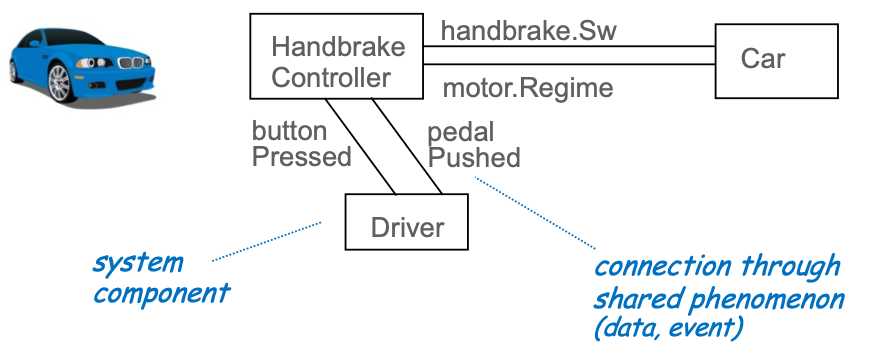
\includegraphics[scale=0.4]{img/context.png}
    \caption{Esempio di Context Diagram}
\end{figure}
\subsubsection{Problem Diagram}
I diagrammi dei problemi sono una forma dettagliata di diagrammi
di contesto che evidenziano i componenti del sistema e le loro interazioni.
Questi diagrammi mostrano chi controlla e monitora i fenomeni condivisi e
indicano i requisiti e i componenti influenzati da essi. 

\begin{figure}[H]
    \centering
    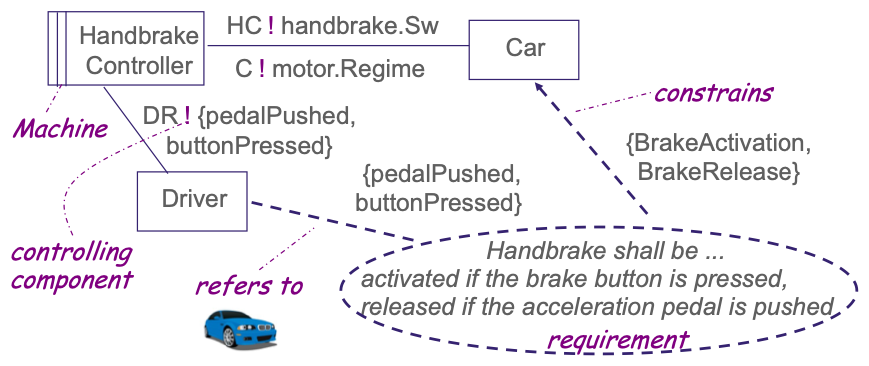
\includegraphics[scale=0.4]{img/problem.png}
    \caption{Esempio di Problem Diagram}
\end{figure}
\subsubsection{Frame Diagram}
I frame diagram sono utilizzati per catturare pattern di problemi frequenti all'interno di un sistema, evidenziando fenomeni tipizzati e componenti tipizzati. Questi diagrammi aiutano a comprendere le interazioni tra i vari elementi del sistema e i requisiti correlati.

\begin{itemize}
    \item \textbf{Fenomeni Tipizzati:}
    \begin{itemize}
        \item \textbf{Causale (C):} Fenomeni che causano effetti diretti.
        \item \textbf{Evento (E):} Fenomeni che rappresentano eventi specifici.
        \item \textbf{Simbolico (Y):} Fenomeni che rappresentano simboli o dati.
    \end{itemize}

    \item \textbf{Componenti Tipizzati:}
    \begin{itemize}
        \item \textbf{Causale (C):} Componenti che causano effetti diretti.
        \item \textbf{Biddable (B):} Componenti che possono essere controllati o influenzati.
        \item \textbf{Lessicale (X):} Componenti che rappresentano dati o informazioni.
    \end{itemize}
\end{itemize}

\begin{figure}[H]
    \centering
    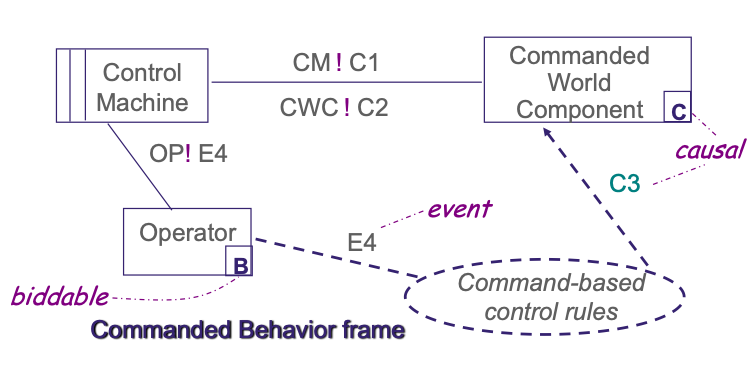
\includegraphics[scale=0.4]{img/frame.png}
    \caption{Esempio di Frame Diagram}
\end{figure}
Un esempio di istanziazione di un frame diagram è il seguente:
\begin{figure}[H]
    \centering
    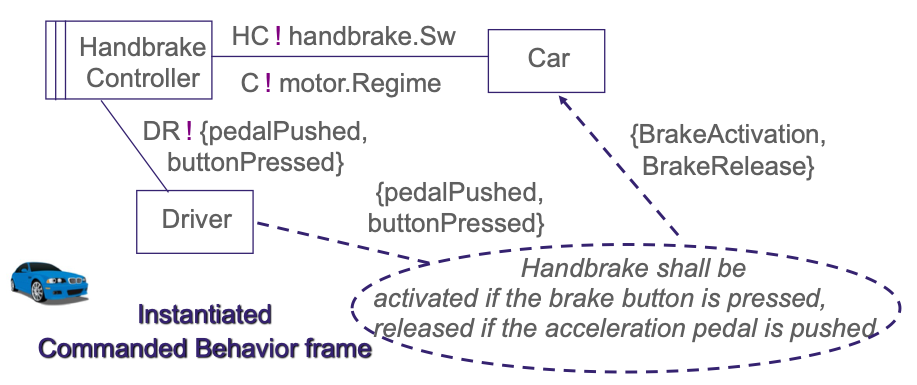
\includegraphics[scale=0.4]{img/instace_frame.png}
    \caption{Esempio di Frame Diagram istanziato}
\end{figure}
\subsection{Diagrammi Entità-Relazione}
I diagrammi Entità-Relazione sono utilizzati per rappresentare le entità e le
relazioni tra di esse in un sistema. Questi diagrammi sono utilizzati per modellare
i dati e le loro interazioni all'interno del sistema, aiutando a definire i requisiti
relativi alla gestione dei dati.

\begin{itemize}
    \item \textbf{Specializzazione delle Entità:} Le entità possono essere
    specializzate in sottoclassi con caratteristiche specifiche (attributi, relazioni).
    Ad esempio, un \textit{ImportantParticipant} eredita attributi e relazioni dalla
    superclass \textit{Participant}, ma può avere attributi aggiuntivi come \textit{Preferences}.
    \item \textbf{Annotazioni dei Diagrammi:} Essenziali per definire con precisione
    gli elementi e evitare errori di specifica. Ad esempio, l'annotazione per
    \textit{Participant} può specificare che è una persona attesa alla riunione in
    un ruolo specifico.
\end{itemize}

\begin{tcolorbox}[colback=red!5!white,colframe=red!75!black,title=Svantaggi dei
    Diagrammi Entità-Relazione]
    Non si riesce a distinguere tra prescrittivi e percettivi.
\end{tcolorbox}
\subsection{Diagrammi \texttt{SADT} (Structured Analytics Design Technique)}
I diagrammi \texttt{SADT} sono utilizzati per catturare attività e dati nel sistema, sia nello stato attuale che in quello futuro. Questi diagrammi si dividono in due categorie principali:

\begin{itemize}
    \item \textbf{Actigram:} Relaziona le attività tramite collegamenti di
    dipendenza dai dati (\textit{input/output}). Mostra come le attività sono correlate
    attraverso i dati che utilizzano e producono.
    \item \textbf{Datagram:} Relaziona i dati tramite collegamenti di dipendenza
    dal controllo (\textit{produttori/consumatori}). Indica come i dati vengono prodotti,
    consumati, validati e le risorse necessarie.
    \begin{itemize}
        \item \textbf{Est:} attività di produzione.
        \item \textbf{Nord:} attività di validazione.
        \item \textbf{Ovest:} attività di consumo.
        \item \textbf{Sud:} risorse necessarie.
    \end{itemize}
\end{itemize}

Nei diagrammi \texttt{SADT}, esiste una dualità dati-attività:
\begin{itemize}
    \item I dati in un actigram devono apparire in un datagram.
    \item Le attività in un datagram devono apparire in un actigram.
\end{itemize}

\begin{tcolorbox}[colback=green!5!white,colframe=green!75!black,title=Vantaggi dei
    Diagrammi \texttt{SADT}]
    \begin{itemize}
        \item Forniscono una chiara visualizzazione delle dipendenze tra attività e dati.
        \item Aiutano a identificare le risorse necessarie e le relazioni di controllo.
    \end{itemize}
\end{tcolorbox}

\begin{tcolorbox}[colback=red!5!white,colframe=red!75!black,title=Svantaggi
    dei Diagrammi \texttt{SADT}]
    \begin{itemize}
        \item Possono diventare complessi e difficili da gestire per sistemi di grandi
        dimensioni.
        \item Richiedono una comprensione approfondita delle attività e dei dati coinvolti.
    \end{itemize}
\end{tcolorbox}

Un esempio di diagramma \texttt{SADT} mostra come le attività di gestione dei vincoli
(\textit{handling constraints}) siano correlate attraverso richieste di meeting,
data range e risorse necessarie. Ogni attività e dato è chiaramente definito
e le loro interazioni sono mappate per garantire la coerenza e la completezza
del sistema.

\subsection{Diagrammi di Flusso dei Dati (\textit{Dataflow Diagrams})}
I diagrammi di flusso dei dati (\texttt{DFD}) sono utilizzati per catturare le operazioni
del sistema collegate dalle dipendenze dei dati. Questi diagrammi sono più semplici
ma meno espressivi rispetto agli actigram.

\begin{itemize}
    \item \textbf{Operazione:} Attività di trasformazione dei dati.
    \item \textbf{Link di Input e Output:} Flussi di dati. Le operazioni richiedono
    dati in entrata per produrre dati in uscita (non flusso di controllo).
    \item \textbf{Regole di Trasformazione dei Dati:} Devono essere specificate nelle
    annotazioni (linguaggio naturale strutturato) o in un altro \texttt{DFD} 
    (raffinamento delle operazioni,
    cf. \texttt{SADT}).
    \item \textbf{Componenti del Sistema e Repositori di Dati:} Origini e destinazioni
    del flusso.
\end{itemize}

\begin{tcolorbox}[colback=green!5!white,colframe=green!75!black,title=Vantaggi dei
    Diagrammi di Flusso dei Dati]
    \begin{itemize}
        \item Semplificano la rappresentazione delle operazioni di trasformazione dei dati.
        \item Facilitano la comprensione delle dipendenze dei dati nel sistema.
    \end{itemize}
\end{tcolorbox}

\begin{tcolorbox}[colback=red!5!white,colframe=red!75!black,title=Svantaggi dei Diagrammi
    di Flusso dei Dati]
    \begin{itemize}
        \item Meno espressivi rispetto agli actigram per rappresentare le operazioni
        complesse.
        \item Richiedono annotazioni dettagliate per specificare le regole di
        trasformazione dei dati.
    \end{itemize}
\end{tcolorbox}

I diagrammi di flusso dei dati sono essenziali per garantire la coerenza e la
completezza del sistema, con ogni attività che deve avere un input e un output,
e tutti i dati devono avere un produttore e un consumatore. Le regole di
consistenza/completa possono essere verificate da strumenti, simili ai diagrammi \texttt{SADT}.
\begin{figure}[H]
    \centering
    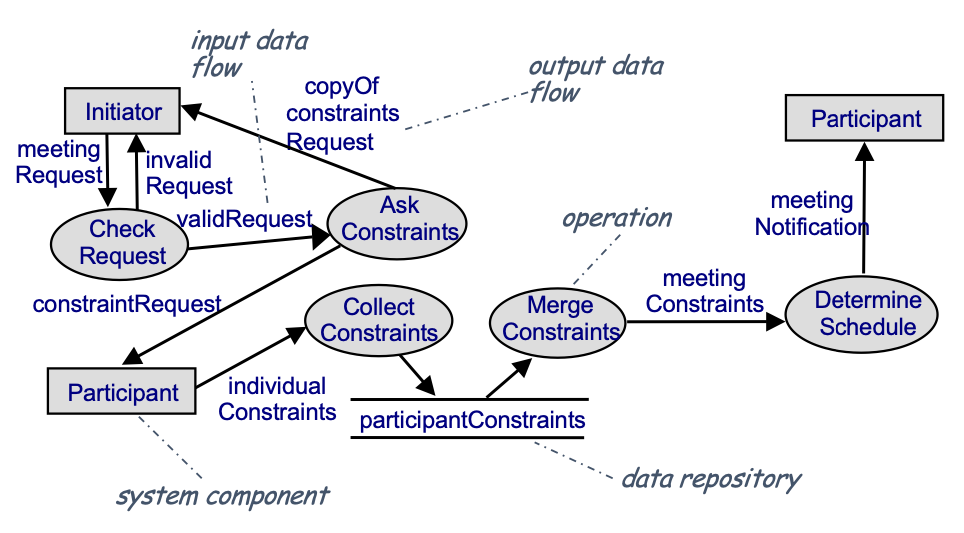
\includegraphics[scale=0.35]{img/dfd.png}
    \caption{Esempio di Diagramma di Flusso dei Dati}
\end{figure}
\subsection{Use Case Diagram}
I diagrammi dei casi d'uso sono utilizzati per catturare le operazioni che devono essere eseguite da un componente del sistema e le interazioni con altri componenti. Questi diagrammi forniscono una vista di insieme semplice ma a volte vaga delle operazioni del sistema.

\begin{itemize}
    \item \textbf{Operazioni del Sistema:} Catturano le operazioni da eseguire
    e le interazioni con altri componenti. Sono introdotti in \texttt{UML} per sostituire i \texttt{DFD}.
    \item \textbf{Annotazioni e Scenari di Interazione:} Necessari per rendere
    precisi i diagrammi dei casi d'uso.
    \item \textbf{Meccanismi di Strutturazione:}
    \begin{itemize}
        \item \texttt{<<include>>}: Specifica una ``sotto-operazione''.
        \item \texttt{<<extend>>} + precondizione: Specifica un'operazione
        ``variante'' in casi eccezionali.
    \end{itemize}
\end{itemize}

\begin{tcolorbox}[colback=green!5!white,colframe=green!75!black,title=Vantaggi
    dei Diagrammi dei Casi d'Uso]
    \begin{itemize}
        \item Forniscono una vista di insieme delle operazioni del sistema.
        \item Facilmente comprensibili anche da stakeholder non tecnici.
    \end{itemize}
\end{tcolorbox}

\begin{tcolorbox}[colback=red!5!white,colframe=red!75!black,title=Svantaggi
    dei Diagrammi dei Casi d'Uso]
    \begin{itemize}
        \item Possono essere troppo vaghi senza annotazioni dettagliate.
        \item Richiedono scenari di interazione per essere completamente utili.
    \end{itemize}
\end{tcolorbox}

I diagrammi dei casi d'uso sono strumenti potenti per la modellazione delle
operazioni del sistema, ma devono essere integrati con annotazioni e scenari
di interazione per garantire una comprensione completa e precisa delle funzionalità
del sistema.
\subsection{Event trace diagrams}
I diagrammi delle tracce degli eventi catturano scenari positivi attraverso
sequenze di interazioni tra istanze dei componenti del sistema. Questi diagrammi
mostrano come le interazioni si svolgono nel tempo.

\begin{tcolorbox}[colback=green!5!white,colframe=green!75!black,title=Vantaggi dei 
    Diagrammi delle Tracce degli Eventi]
    \begin{itemize}
        \item Permettono di visualizzare chiaramente le interazioni tra i componenti 
        del sistema.
        \item Forniscono una sequenza temporale dettagliata degli eventi di interazione.
    \end{itemize}
\end{tcolorbox}

\begin{tcolorbox}[colback=red!5!white,colframe=red!75!black,title=Svantaggi dei 
    Diagrammi delle Tracce degli Eventi]
    \begin{itemize}
        \item Possono diventare complessi con un numero elevato di componenti e interazioni.
        \item Richiedono una comprensione dettagliata delle sequenze di interazione.
    \end{itemize}
\end{tcolorbox}
\subsection{State Machine Diagram}
I diagrammi delle macchine a stati catturano i comportamenti ammissibili dei componenti del sistema. Essi rappresentano la sequenza delle transizioni di stato per gli elementi controllati.

\begin{itemize}
    \item \textbf{Comportamento di un'istanza di componente:} Sequenza di transizioni di
    stato per gli elementi che controlla.
    \item \textbf{Stato della Macchina a Stati:} Insieme di situazioni in cui una variabile
    che caratterizza un elemento controllato ha sempre lo stesso valore. Ad esempio,
    lo stato ``MeetingScheduled'' ha sempre lo stesso valore per ``Date'' e ``Location''.
    \item \textbf{Stati Iniziali e Finali:} Stati in cui l'elemento appare o scompare.
    Gli stati possono avere una certa durata.
    \item \textbf{Transizione di Stato della Macchina a Stati:} Causata da un evento
    associato. Se l'elemento è nello stato di origine e l'evento si verifica, allora passa allo stato di destinazione. Gli eventi sono fenomeni istantanei.
\end{itemize}

\begin{tcolorbox}[colback=green!5!white,colframe=green!75!black,title=Vantaggi dei
    Diagrammi delle Macchine a Stati]
    \begin{itemize}
        \item Permettono di modellare chiaramente i comportamenti ammissibili dei
        componenti del sistema.
        \item Forniscono una rappresentazione dettagliata delle transizioni di stato.
    \end{itemize}
\end{tcolorbox}

\begin{tcolorbox}[colback=red!5!white,colframe=red!75!black,title=Svantaggi dei
    Diagrammi delle Macchine a Stati]
    \begin{itemize}
        \item Possono diventare complessi con un numero elevato di stati e transizioni.
        \item Richiedono una comprensione dettagliata dei comportamenti dei componenti.
    \end{itemize}
\end{tcolorbox}
Per evitare l'esplosione combinatoria di stati è possibile utilizzare gli statecharts,
che permettono di modellare comportamenti complessi in modo più chiaro e conciso.
\begin{figure}[H]
    \centering
    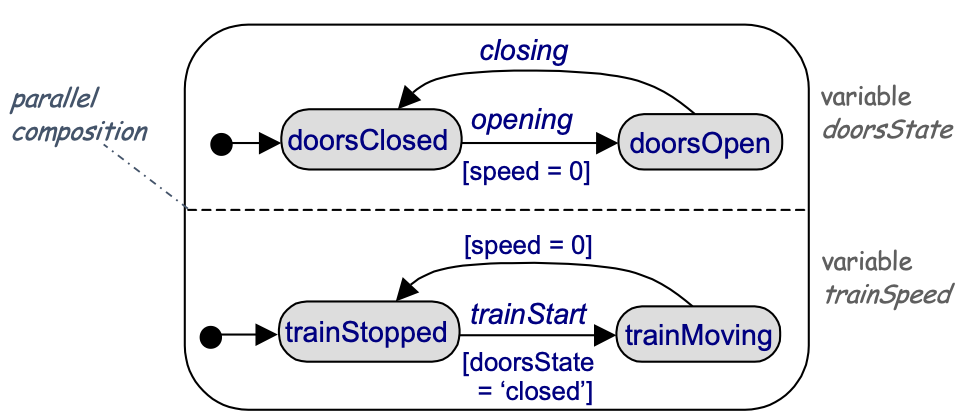
\includegraphics[scale=0.3]{img/statechart.png}
    \caption{Esempio di State Machine Diagram}
\end{figure}
\subsection{\texttt{R-net} Diagram}
Se vogliamo ragionare in termini di stimolo e risposta agli stimoli, 
una versione alternativa è il diagramma \texttt{R-net}, che cattura le relazioni
tra gli stimoli provenienti da un'entità esterna e le risposte generate dal sistema.
\begin{figure}[H]
    \centering
    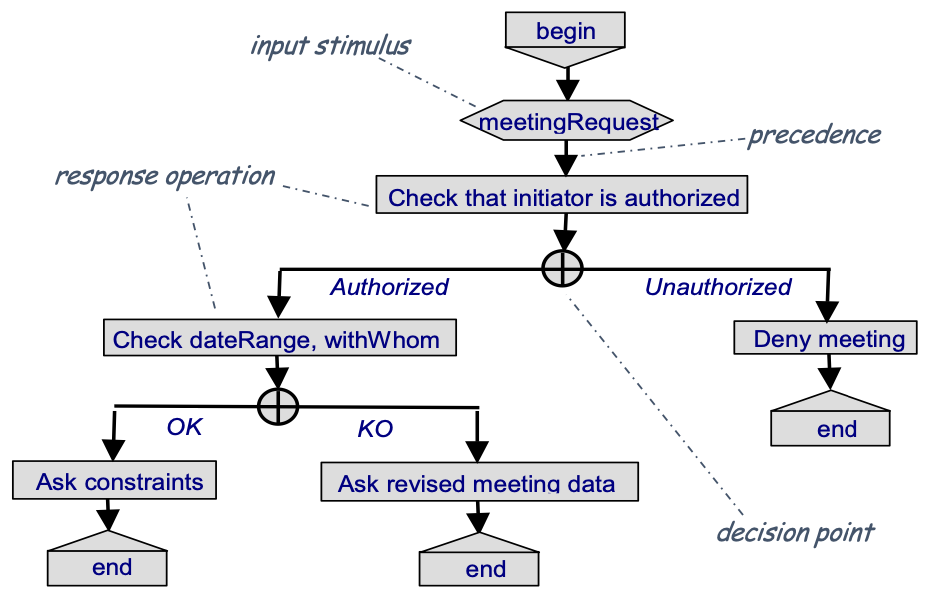
\includegraphics[scale=0.4]{img/rnet.png}
    \caption{Esempio di R-net Diagram}
\end{figure}
\section{Integrare i Diagrammi in un sistema multi-vista}
Avendo a disposizione una varietà di diagrammi per
rappresentare i requisiti del sistema, possiamo integrare i diversi diagrammi dato 
che ciascuno fornisce una prospettiva unica sul sistema. 
Una prima verifica, data dai sistemi automatici, può essere fatta per verificare
la consistenza tra i diagrammi. 

Le inconsistenze che si possono verificare possono essere diverse, tra cui:
\begin{itemize}
    \item tutti i componenti di un problem diagram devono essere presenti
    in un diagramma entità-relazione.
    \item tutti i fenomeni di un problem diagram devono essere presenti
    in un diagramma entità-relazione come un'entità, un attributo o una relazione.
\end{itemize}

Ci sono viste alternative in \texttt{UML} che ci permetto di ragionare, non tanto 
sull'architettura, ma supportano nella fasi di progettazione e validazione dei requisiti,
come ad esempio:
\begin{itemize}
    \item \textbf{Diagrammi delle Classi}: utili per la vista strutturale del sistema.
    \item \textbf{Use Case Diagram}: utile per la vista operazionale del sistema.
    \item \textbf{Sequence Diagram}: utile per la visione degli scenari.
    \item \textbf{State Diagram}: utile per la visione delle state machine.
\end{itemize}

\begin{tcolorbox}[colback=green!5!white,colframe=green!75!black,title=Vantaggi
    dell'ausilio di Diagrammi]
    \begin{itemize}
        \item Sono diversi dalla presentazione in linguaggio naturale, permettendo
        quindi di essere guidati.
        \item Hanno una semantica precisa, non ambigua.
        \item Mezzo di informazione più funzionale per il dialogo con gli stakeholder.
        \item Hanno una struttura grafica che permette di avere una panoramica di 
        alto livello.
        \item Sono facili da capire e da comunicare.
        \item Permettono di fare un'analisi di primo livello e sono supportati da tool.
    \end{itemize}
\end{tcolorbox}
\begin{tcolorbox}[colback=red!5!white,colframe=red!75!black,title=Svantaggi
    dell'ausilio di Diagrammi]
    \begin{itemize}
        \item Il linguaggio semantico può essere vago (\textit{con interpretazioni differenti}).
        \item Spesso vengono formalizzati solo gli aspetti più evidenti e superficiali del
        sistema, lasciando non formalizzate le proprietà dettagliate degli
        elementi, il che può limitare la profondità dell'analisi.
        \item L'analisi automatizzata è limitata.
        \item Si modellano solo aspetti funzionali e strutturali.
    \end{itemize}
\end{tcolorbox}
Le specifiche più formali sono richieste per sistemi \textit{mission critical}.
\chapter{Validazione e verifica}
L'obiettivo di tale fare è quella di partire da un documento dei 
requisiti consolidato e di verificare che esso sia corretto e completo.

Alcuni errori siamo stati in grado di evitarli in partenza, grazie alle fasi 
precedenti. In questa fase ci concentriamo nell'individuazione di errori
che non sono stati individuati in precedenza. 

Il primo obiettivo è la \textbf{ricerca} che si divide in tre fasi.
La prima fase da seguire è la \textbf{validazione}, che consiste nel verificare 
che il documento dei requisiti soddisfi le esigenze del cliente.
La seconda fase è la \textbf{verifica}, che consiste nel verificare che il
documento sia corretto e completo.
La terza fase è la \textbf{controllo}, che riguarda il raggiungimento 
tei target di qualità.

Il secondo obiettivo è la \textbf{documentazione} dei difetti, che include 
anche l'\textbf{analisi} delle cause e la loro correzione.

\begin{tcolorbox}[colback=orange!5!white,colframe=orange!75!black,title=Output della fase]
    L'output di tale fase è la versione finale del documento dei requisiti.
    
    Oltre a tale documento possiamo considerare anche i test di accettazione consolidati, 
    eventualmente un prototipo, un piano di sviluppo e potenzialmente un contratto.
\end{tcolorbox}

\section{Come si affronta la revisione}
\subsection{Ispezione e revisione}
L'idea è quella di avere uno o più esperti che prendono il documento dei requisiti
che prendono il documento dei requisiti e lo analizzano oppure utilizzare dei meeting 
di gruppo per discutere il documento.

Principalmente si utilizzano due tecniche:
\begin{itemize}
    \item \textbf{Walkthrough}: si tratta di una lettura del documento,
    con l'obiettivo di trovare errori.
    \item \textbf{Più strutturato}: utilizzando degli ispettori esterni, dei 
    meeting ben strutturati, report o altro.
\end{itemize}

Un processo che mira ad assicurare la qualità del documento dei requisiti segue tali fasi:
\begin{figure}[H]
    \centering
    \begin{tikzpicture}
        % Styles
        \tikzstyle{process} = [rectangle, rounded corners, 
        minimum width=3cm, minimum height=1cm, text centered, draw=black, 
        fill=blue!20, text width=2.5cm]
      
        % Nodes
        \node (start) [circle, fill, inner sep=2pt] {};
        \node (identify) [process, right=0.5cm of start]
        {Pianificare \\ l'Ispezione del \\ Documento};
        \node (detect) [process, right=0.5cm of identify]
        {Revisione \\ individuale};
        \node (generate) [process, right=0.5cm of detect]
        {Valutazione \\ dei difetti};   
        \node (evaluate) [process, right=0.5cm of generate]
        {Consolidamento del \\ Documento dei \\ Requisiti};
      
        % Arrows
        \draw[->] (start) -- (identify);
        \draw[->] (identify) -- (detect);
        \draw[->] (detect) -- (generate);
        \draw[->] (generate) -- (evaluate);
        \draw[->]  (evaluate.south) -- ++(0,-0.5) -| (start.south);
    \end{tikzpicture}
\end{figure}
\begin{itemize}
    \item \textbf{Pianificare l'ispezione del documento}: si tratta di definire
    chi sono gli ispettori, come si svolgerà l'ispezione, quali sono gli obiettivi
    e quali sono i criteri di accettazione.
    \item \textbf{Revisione individuale}: ogni ispettore legge il documento e
    cerca di individuare errori.
    Tale fase può seguire diverse modalità:
    \begin{itemize}
        \item Liberamente: ogni ispettore legge il documento e cerca di individuare
        errori.
        \item Guidata mediante checklist: ogni ispettore segue una lista di controllo
        basata sul dominio.
        \item Basato sul processo.
    \end{itemize}
    \item \textbf{Valutazione dei difetti}: si tratta di valutare i difetti
    capendo come sono stati generati e come possono essere corretti.
    \item \textbf{Consolidamento del documento dei requisiti}: si tratta della 
    fase in cui viene consolidato il documento dei requisiti.
\end{itemize}
Tale processo può essere ripetuto più volte, fino a quando non si è soddisfatti
della qualità del documento.
\subsection{Linee guida per la revisione}
\begin{itemize}
    \item \textbf{Rapporto di Ispezione:}
    \begin{itemize}
        \item Deve essere \textit{informativo}, \textit{accurato} e \textit{costruttivo}.
        \item Non deve contenere opinioni personali o commenti che possano risultare 
        offensivi.
        \item Deve seguire una \textit{struttura standard} che permetta l'aggiunta 
        di commenti liberi e sia di facile lettura.
        \item Può servire da guida per la revisione individuale.
    \end{itemize}
    
    \item \textbf{Gli Ispettori:}
    \begin{itemize}
        \item Devono essere \textit{indipendenti} dagli autori del documento sotto 
        revisione.
        \item Devono rappresentare tutti gli \textit{stakeholder} e provenire da 
        \textit{background diversi}.
    \end{itemize}
    
    \item \textbf{Tempistica dell'Ispezione:}
    \begin{itemize}
        \item L'ispezione non deve avvenire né \textit{troppo presto} né 
        \textit{troppo tardi}.
        \item Incontri \textit{brevi} e \textit{ripetuti} risultano più efficaci.
    \end{itemize}
    
    \item \textbf{Focus Maggiore su Parti Critiche:}
    \begin{itemize}
        \item Maggiore è il numero di difetti in una parte, maggiore deve essere 
        lo \textit{scrutinio} su quella parte.
    \end{itemize}
\end{itemize}
\subsection{Checklist}
L'obiettivo principale delle liste di controllo per l'ispezione è di dirigere 
la ricerca dei difetti verso specifiche problematiche, migliorando così 
l'efficienza e l'efficacia del processo di revisione. Le liste di controllo 
si suddividono in diverse categorie, ognuna con un focus particolare:

\begin{itemize}
    \item \textbf{Liste basate sui difetti:} Queste liste comprendono domande 
    generiche che sono strutturate in base al tipo di difetto. L'intento è di 
    coprire un ampio spettro di possibili anomalie in modo organizzato.

    \item \textbf{Liste specifiche per qualità:} Tali liste affinano le domande 
    delle liste basate sui difetti per concentrarsi su specifiche categorie di 
    requisiti non funzionali (NFR), come la sicurezza, la performance e 
    l'usabilità. Queste liste possono anche essere basate su parole guida e 
    sono frequentemente orientate a identificare omissioni, migliorando così 
    la completezza del software o del prodotto analizzato.

    \item \textbf{Liste specifiche per dominio:} Queste liste rappresentano 
    un'ulteriore specializzazione e si concentrano sui concetti e le operazioni 
    specifici di un dominio. Sono particolarmente utili per offrire una guida 
    dettagliata nella ricerca di difetti, assicurando che le peculiarità del 
    dominio siano adeguatamente considerate.

    \item \textbf{Liste basate sul linguaggio:} Queste liste adattano le liste 
    basate sui difetti ai costrutti di linguaggi di specifica particolari, 
    supportando processi di automazione. La ricchezza dei linguaggi di specifica 
    consente implementazioni di controlli più sofisticati e mirati.
\end{itemize}
\begin{tcolorbox}[colback=green!5!white,colframe=green!75!black,title=Vantaggi 
    delle Checklist]
    \begin{itemize}
      \item \textbf{Maggiore efficacia rispetto all'ispezione del codice:} Utilizzo 
      di un modello basato su processi che combina checklist basate sui difetti, 
      specifiche per qualità e specifiche per linguaggio, risultando estremamente efficace.
      \item \textbf{Ampia applicabilità:} Adatte per ogni tipo di difetto e formato 
      di specifica, rendendole strumenti versatili.
    \end{itemize}
    \end{tcolorbox}
    
    \begin{tcolorbox}[colback=red!5!white,colframe=red!75!black,title=Limitazioni 
        delle Checklist]
    \begin{itemize}
      \item \textbf{Onere e costo del processo di ispezione:} La dimensione del 
      materiale di ispezione e il tempo/costo necessari per gli ispettori esterni 
      e le riunioni di revisione possono essere significativi.
      \item \textbf{Nessuna garanzia di rilevare tutti i difetti importanti:} Nonostante 
      l'efficacia, le checklist non possono garantire il rilevamento di tutti i 
      difetti critici.
    \end{itemize}
    \end{tcolorbox}
\section{Approccio guidato da Query}
La quality assurance può essere vista come delle particolari interrogazioni a 
delle strutture dati. Tipicamente le query possono essere formulate in presenza di una documentazione 
strutturata dei requisti. Per strutturata intendiamo una documentazione che
si basa su diagrammi.

Quando si formulano tali query utilizzando i \texttt{CASE} tools, si possono
ottenere delle risposte automatiche.
\section{Validazione dei requisiti mediante animazioni}
L'obiettivo principale di questa metodologia è verificare l'adeguatezza dei requisiti 
rispetto alle reali necessità degli utenti. Questo processo può essere attuato 
attraverso due approcci principali:

\subsubsection{Approccio 1: Visualizzazione di Scenari di Interazione}
Questo approccio consiste nel mostrare scenari di interazione concreti in azione, 
utilizzando strumenti di attuazione sui diagrammi di Evento Tempo (\texttt{ET}). Tuttavia, 
questo metodo presenta sfide legate alla copertura completa degli scenari, che 
può risultare incompleta.

\subsubsection{Approccio 2: Utilizzo di Strumenti di Animazione delle Specifiche}
L'animazione delle specifiche si svolge in quattro fasi principali:
\begin{enumerate}
    \item \textbf{Generazione del Modello Esecutivo:} Si estrae o si genera un 
    modello eseguibile direttamente dalle specifiche tecniche.
    \item \textbf{Simulazione del Comportamento:} Il sistema viene simulato 
    basandosi su questo modello, dove eventi stimolo vengono inviati per imitare 
    il comportamento dell'ambiente circostante e si osserva la risposta del modello.
    \item \textbf{Visualizzazione della Simulazione:} La simulazione viene 
    visualizzata mentre è in corso, permettendo una valutazione immediata e 
    dinamica del comportamento del sistema.
    \item \textbf{Feedback degli Utenti:} I feedback degli utenti vengono 
    raccolti e analizzati per valutare l'efficacia della simulazione e del 
    modello proposto.
\end{enumerate}
\begin{tcolorbox}[colback=green!5!white,colframe=green!75!black,title=Punti di Forza]
    \begin{itemize}
      \item \textbf{Verifica dell'Adeguazione:} Metodo efficace per controllare 
      l'adeguatezza dei requisiti rispetto alle necessità reali e all'ambiente attuale.
      \item \textbf{Coinvolgimento degli Stakeholder:} Il principio ``WYSIWYC" 
      (What You See Is What You Check) permette ai stakeholder di visualizzare e 
      verificare i requisiti direttamente.
      \item \textbf{Estensione a Controesempi:} Possibilità di animare controesempi 
      generati da altri strumenti come i verificatori di modelli, migliorando così la robustezza del sistema.
      \item \textbf{Riutilizzo degli Scenari:} Gli scenari di animazione possono 
      essere conservati per replay futuri e usati come dati di test di accettazione.
    \end{itemize}
    \end{tcolorbox}
    
    \begin{tcolorbox}[colback=red!5!white,colframe=red!75!black,title=Limitazioni]
    \begin{itemize}
      \item \textbf{Problema della Copertura:} La progettazione degli scenari deve 
      essere attentamente gestita per assicurare che non vengano tralasciati problemi significativi. Non vi è garanzia di identificare tutti i difetti importanti.
      \item È necessaria una specifica formale 
      dettagliata per eseguire un'animazione efficace dei requisiti, richiedendo 
      un investimento considerevole in termini di tempo e risorse.
    \end{itemize}
\end{tcolorbox}
\end{document}
